\documentclass{article}

\title{Document Title}

\date{Month\\day\\year}

\author{Aaron Jencks\\Electronics Technology Technician Intern, JET Engineering}


\usepackage{pgfplots}

\usepackage{graphicx}

\usepackage{media9}

\usepackage{listings}

\usepackage{hyperref}

\hypersetup{
	colorlinks=true,
	linkcolor=blue,
	filecolor=magenta,
	urlcolor=cyan,
}



\begin{document}

	\maketitle
	\newpage
	\tableofcontents
	\newpage

	

	\section{Summary}
		This test will show how accurate the depth perception of the D435 Intel Realsense camera is when looking vertically down at a flat and unflat surface.
	
	\section{Part 1}
		\subsection{Setup}
	
			\subsubsection{Materials}
	
				\begin{enumerate}
					\item Intel Realsense D435 depth camera
					\item Mounting bracket
					\item A Hydraulic lift to move the camera up and down
					\item Tape measure
					\item Wooden blocks
				\end{enumerate}
	
			\newpage
			\subsubsection{Our Setup}
				We mounted the camera using a clamp and the same mounting system we've used in the other tests and mounted it facing the floor on a hydraulic cart. In order to make it easier to measure I lined the bottom of the camera up with the bottom edge of the platform on the cart. I set the cart to 18 inches from the ground using the tape measure.
	
				
	
				\begin{figure}[h]
					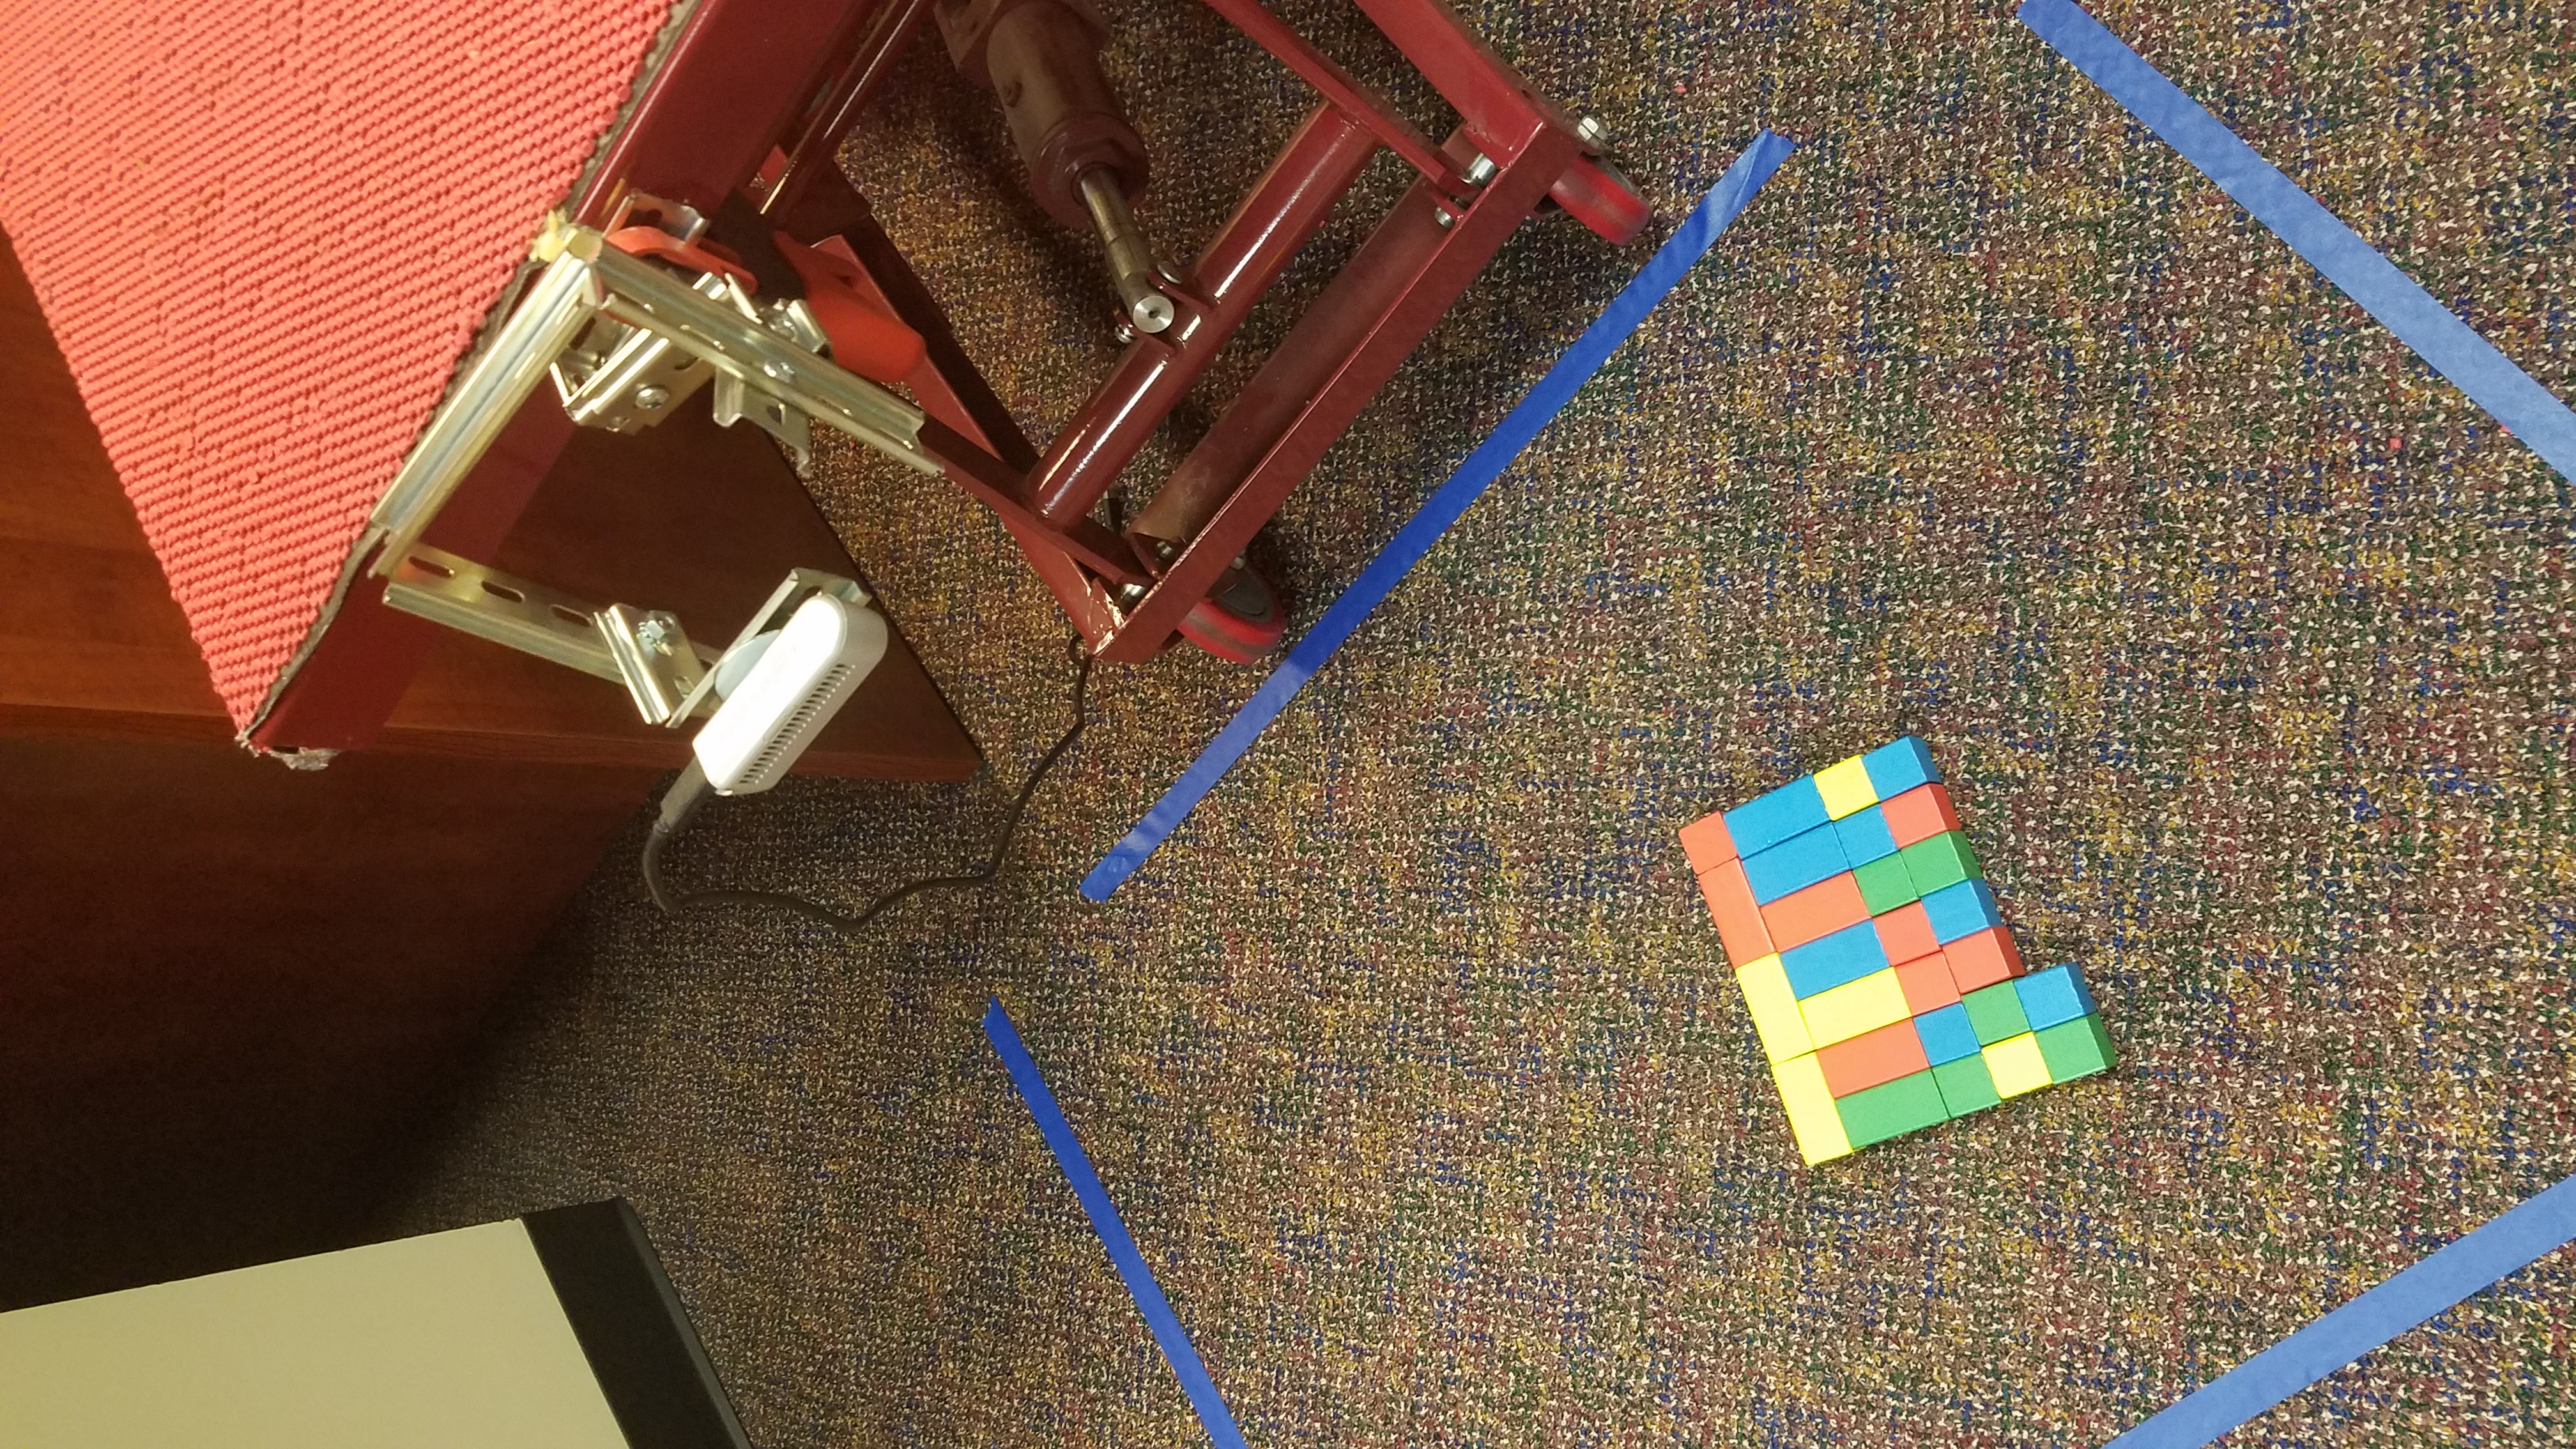
\includegraphics[angle=270, origin=c, height=8cm]{./images/our_setup.jpg}
					\centering
					\caption{Our setup}
					\label{fig:p1_setup}
				\end{figure}
	
				
		\newpage
		\subsection{Process}
			\begin{enumerate}
				\item Reset the cart height to 18 inches, for this baseline, do not place any blocks on the floor
				\item Collect the average depth, using the python program, and record it in excel
				\item Raise the cart by 1 inch
				\item Repeat steps 2-3 until you reach a height of 27 inches
				\item Now place blocks on the floor and spread them around so no two blocks are within 2-3 inches of each other.
				\item Repeat steps 2-4
				\item Now place the blocks in a single mass near the center of the camera view, see Figure \ref{fig:setup}
				\item Repeat steps 2-4
			\end{enumerate}
	
		\newpage
		\subsection{Results}
			Below are images of our results:
			
			\begin{figure}[h]
				\includegraphics[width=8cm]{./images/part_1/actual_error.png}
				\centering
				\caption{Actual Error}
				\label{fig:p1_results_err_actual}
			\end{figure}
		
			\begin{figure}[h]
				\includegraphics[width=8cm]{./images/part_1/average_error.png}
				\centering
				\caption{Average Error}
				\label{fig:p1_results_err_average}
			\end{figure}
		

		\newpage
		\subsubsection{Discussion}
			\paragraph{Edge Smoothing}
			From the data collected, we concluded that the camera is smoothing edges, and as the number of edges it has to smooth decreases, the error decreases; hence why when we clumped the blocks together it increased the depth accuracy versus when the blocks were scattered. See the two images below for examples:
			
			\begin{figure}[h]
				\includegraphics[width=8cm]{./images/part_1/scattered.png}
				\centering
				\caption{Scattered 3D Perception}
				\label{fig:p1_discussion_scattered}
			\end{figure}
			
			\begin{figure}[h]
				\includegraphics[width=8cm]{./images/part_1/clumped.png}
				\centering
				\caption{Clumped 3D Perception}
				\label{fig:p1_discussion_clumped}
			\end{figure}
			
			\paragraph{The Average Depth is Proportional to the Terrain}
			If we place blocks onto the terrain, the average perceived depth got closer to the camera, this is something we expected, and the data confirms.
			
			
	\section{Part 2}
		\subsection{Setup}
		
			\subsubsection{Materials}
			
			\begin{enumerate}
				\item Intel Realsense D435 depth camera
				\item Mounting bracket
				\item A Hydraulic lift to move the camera up and down
				\item Tape measure
				\item Wooden blocks
				\item Painter's Tape
			\end{enumerate}
		
			\newpage
			\subsubsection{Our Setup}
			We mounted the camera using a clamp and the same mounting system we've used in the other tests and mounted it facing the floor on a hydraulic cart. In order to make it easier to measure I lined the bottom of the camera up with the bottom edge of the platform on the cart. I set the cart to 16 inches from the ground using the tape measure.
			
			
			
			\begin{figure}[h]
				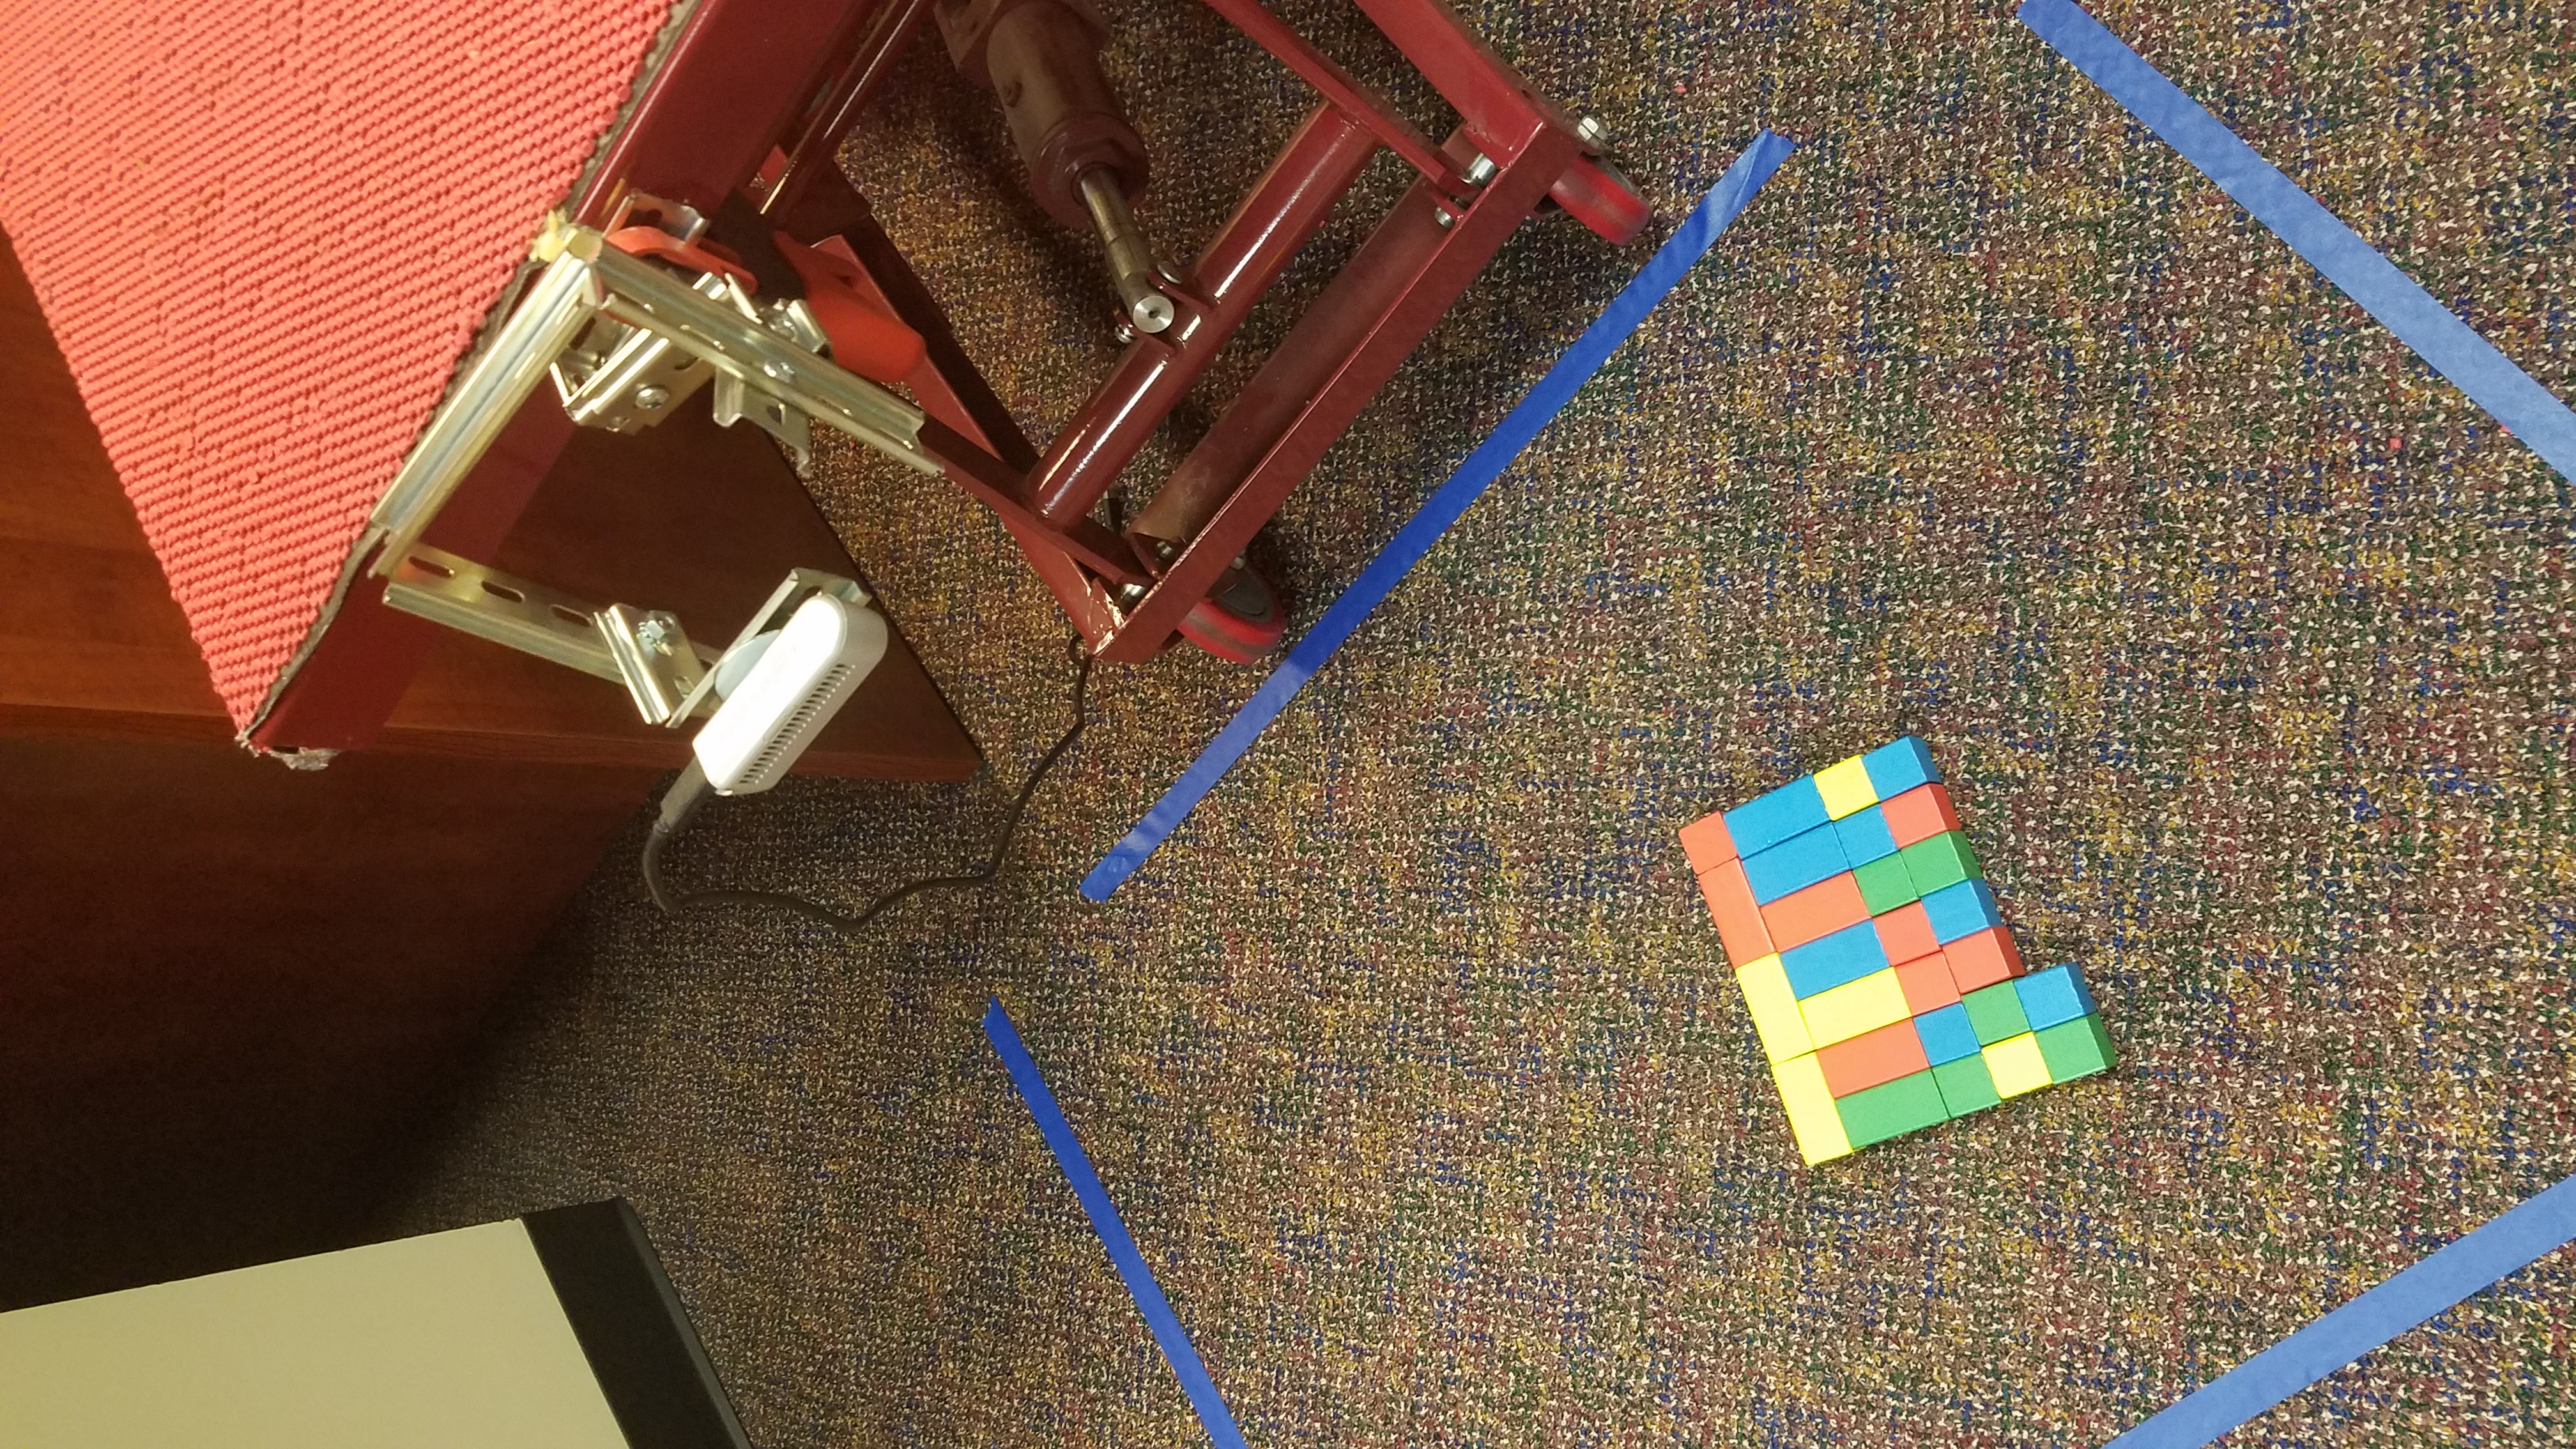
\includegraphics[angle=270, origin=c, height=8cm]{./images/our_setup.jpg}
				\centering
				\caption{Our setup}
				\label{fig:p2_setup}
			\end{figure}
		
		
		\newpage
		\subsection{Process}
			\begin{enumerate}
				\item Reset the cart height to 16 inches, for this baseline, do not place any blocks on the floor
				\item Mark out the field of view on the floor using the painter's tape
				\item Collect the average depth, using the python program, and record it in excel
				\item Add in the blocks in the desired layout, do not use the same layout multiple times
				\item Repeat steps 3-4 until you've collected 20 samples, including the baseline
				\item Now raise the cart to 27 inches
				\item Repeat steps 3-5
			\end{enumerate}
		
		\newpage
		\subsection{Results}
			Below are images of our results:
			
			\begin{figure}[h]
				\includegraphics[width=8cm]{./images/part_2/error_ranges_raw.png}
				\centering
				\caption{Actual Error Percentage Spread}
				\label{fig:p2_results_err_actual}
			\end{figure}
			
			\begin{figure}[h]
				\includegraphics[width=8cm]{./images/part_2/error_ranges_all.png}
				\centering
				\caption{Depth Data Spread}
				\label{fig:p2_results_depth_actual}
			\end{figure}
		
			\newpage
			\begin{figure}[h]
				\includegraphics[width=8cm]{./images/part_2/error_range_16.png}
				\centering
				\caption{Depth Data Spread for 16" Depth}
				\label{fig:p2_results_depth_16}
			\end{figure}
			
			\begin{figure}[h]
				\includegraphics[width=8cm]{./images/part_2/error_range_27.png}
				\centering
				\caption{Depth Data Spread for 27" Depth}
				\label{fig:p2_results_depth_27}
			\end{figure}
		
		
		\newpage
		\subsubsection{Discussion}
			\paragraph{Error and Sensitivity Decrease as Depth Increases}
			From the data we collected, we can conclude that the error is less at lower depths, but is affected greater by rough terrain (see Figure \ref{fig:p2_results_depth_16} and Figure \ref{fig:p2_results_depth_27}).
			
			\paragraph{The Camera is Less Sensitive Near the Edges of the Field of View}
			You can see that the error for these trials dips, indicating that the camera did not detect as much of a change in depth, pushing the average depth closer to the actual reading. This did not seem to have the same effect at 27".
			
			\paragraph{Depth Values Skew Linearly as Depth Increases}
			I also noted that the actual depth value may skew from the correct value as depth increases, this coming from Figure \ref{fig:p2_results_depth_16} the baseline is 16.02 and in Figure \ref{fig:p2_results_depth_27} the baseline is 27.40, a 0.38" increase in distance from the target depth.

	\newpage

	\listoffigures

\end{document}